\documentclass[../main.tex]{subfiles}
\graphicspath{{\subfix{../figures/}}}

\begin{document}
\section{实验工具}
\begin{enumerate}
  \item \texttt{esp8266\_deauther}: 来自
    \url{https://github.com/SpacehuhnTech/esp8266_deauther}.
  \item \textt{Arduino IDE}: 介绍见下文. 我们主要使用它的编译功能,
    生成可执行的二进制文件.
  \item \texttt{安信可串口调试助手}: Windows 和 ESP8266 WiFi 模块交互的界面.
  \item \texttt{Flash Download Tool}: 用于将编译生成的二进制文件下载到 ESP8266
    WiFi 模块.
\end{enumerate}
%
\subsection*{esp8266\_deauther}
\begin{figure}[H]
  \begin{center}
    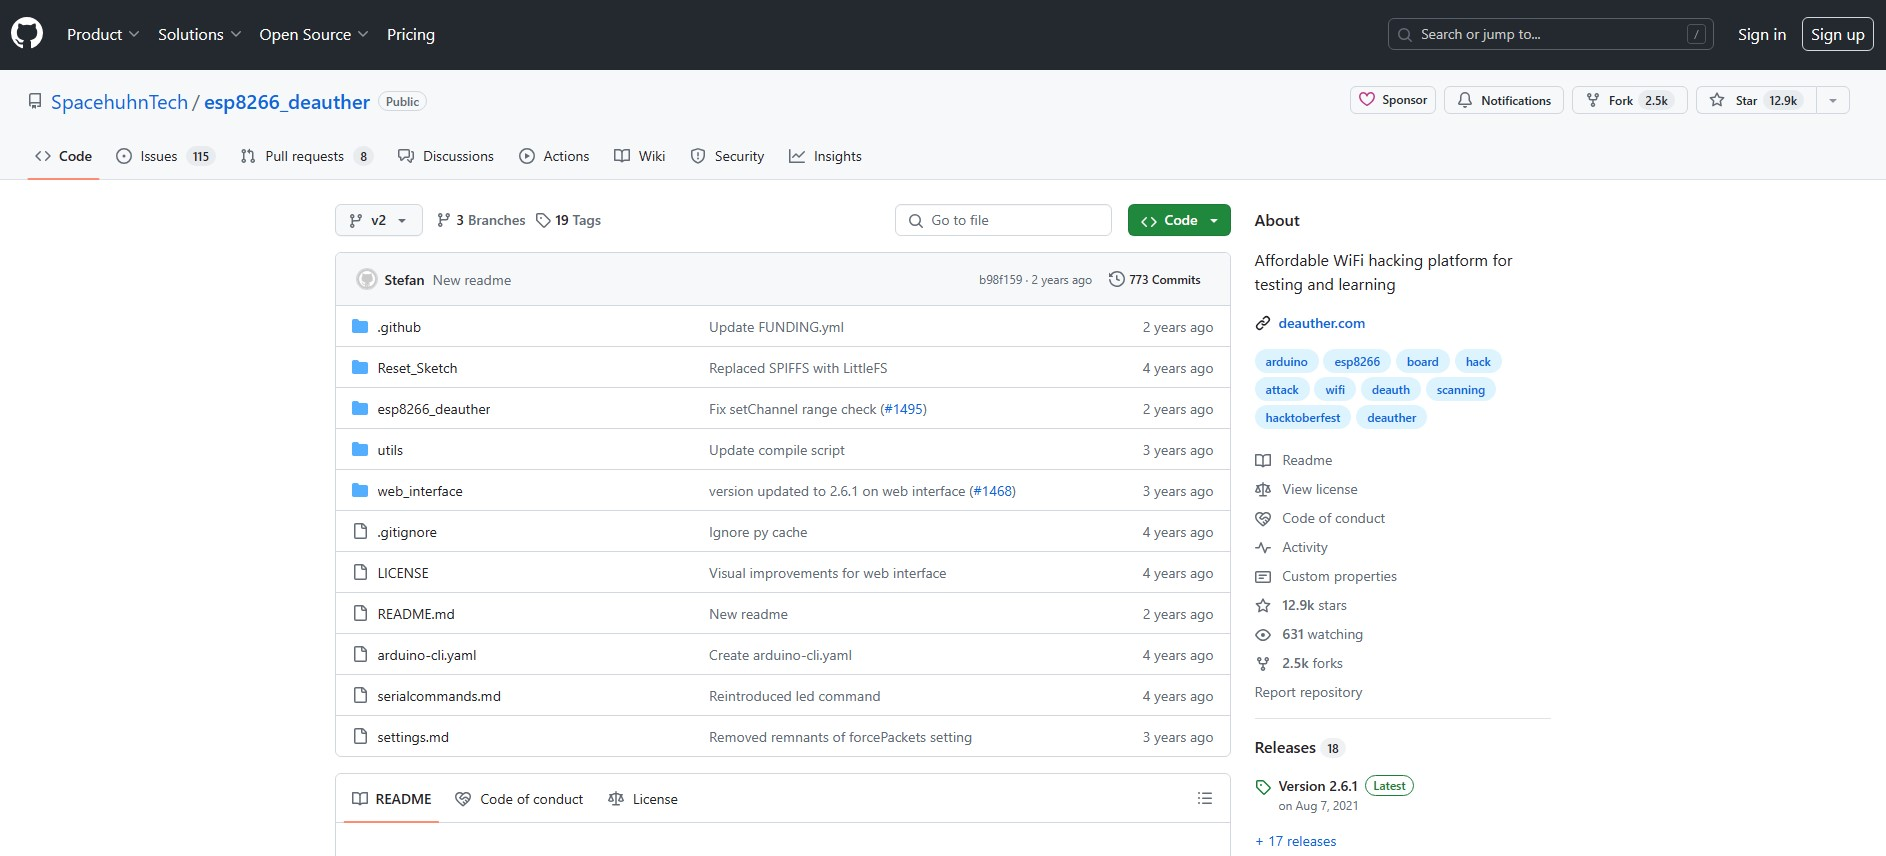
\includegraphics[width=0.55\textwidth]{esp8266_deauther_github_files.jpg}
    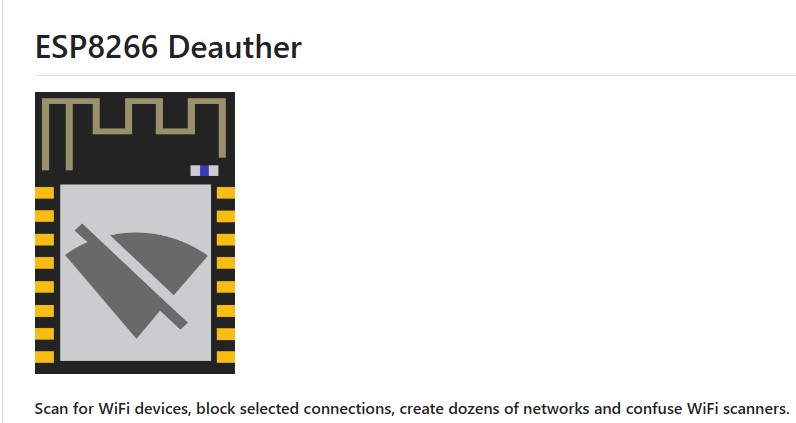
\includegraphics[width=0.35\textwidth]{esp8266_deauther_github_logo.jpg}
  \end{center}
  \caption{Open Source Project: \texttt{esp8266\_deauther}}
\end{figure}
%
\texttt{esp8266\_deauther} 是一个基于 ESP8266 WiFi 模块开发的开源项目,
旨在实现对无线网络中设备进行 Deauthentication(Deauth)攻击的工具。
通过 \texttt{esp8266\_deauther},用户可以利用 ESP8266 WiFi 模块向目标设备发送伪造的 Deauthentication 帧,
从而迫使目标设备与Wi-Fi网络断开连接,造成网络服务中断或干扰。

一般来说,Deauth 攻击是一种无线网络安全测试中常见的方法,
用于验证网络的弱点并评估其韧性。\texttt{esp8266\_deauther} 提供了一个简单但功能强大的方式,
让用户能够轻松地进行 Deauth 攻击,以便测试网络设备的响应能力、
网络流量控制和安全性。

下面是 \texttt{esp8266\_deauther} 的一些特点:
\begin{itemize}
  \item 易用性:\texttt{esp8266\_deauther} 提供了直观的用户界面,
    用户可以通过简单的操作选择目标设备并执行 Deauth 攻击。
  \item 多功能性:除了进行 Deauth 攻击之外,
    \texttt{esp8266\_deauther} 还可能包含其他功能,如监视无线网络流量、
    嗅探数据包等。
  \item 社区支持:作为一个开源项目,\texttt{esp8266\_deauther} 可能受到活跃的开发者社区支持,
    用户可以获取更新、修复漏洞和参与功能改进。
\end{itemize}
%
\subsection*{Arduino IDE}
\begin{figure}[H]
  \begin{center}
    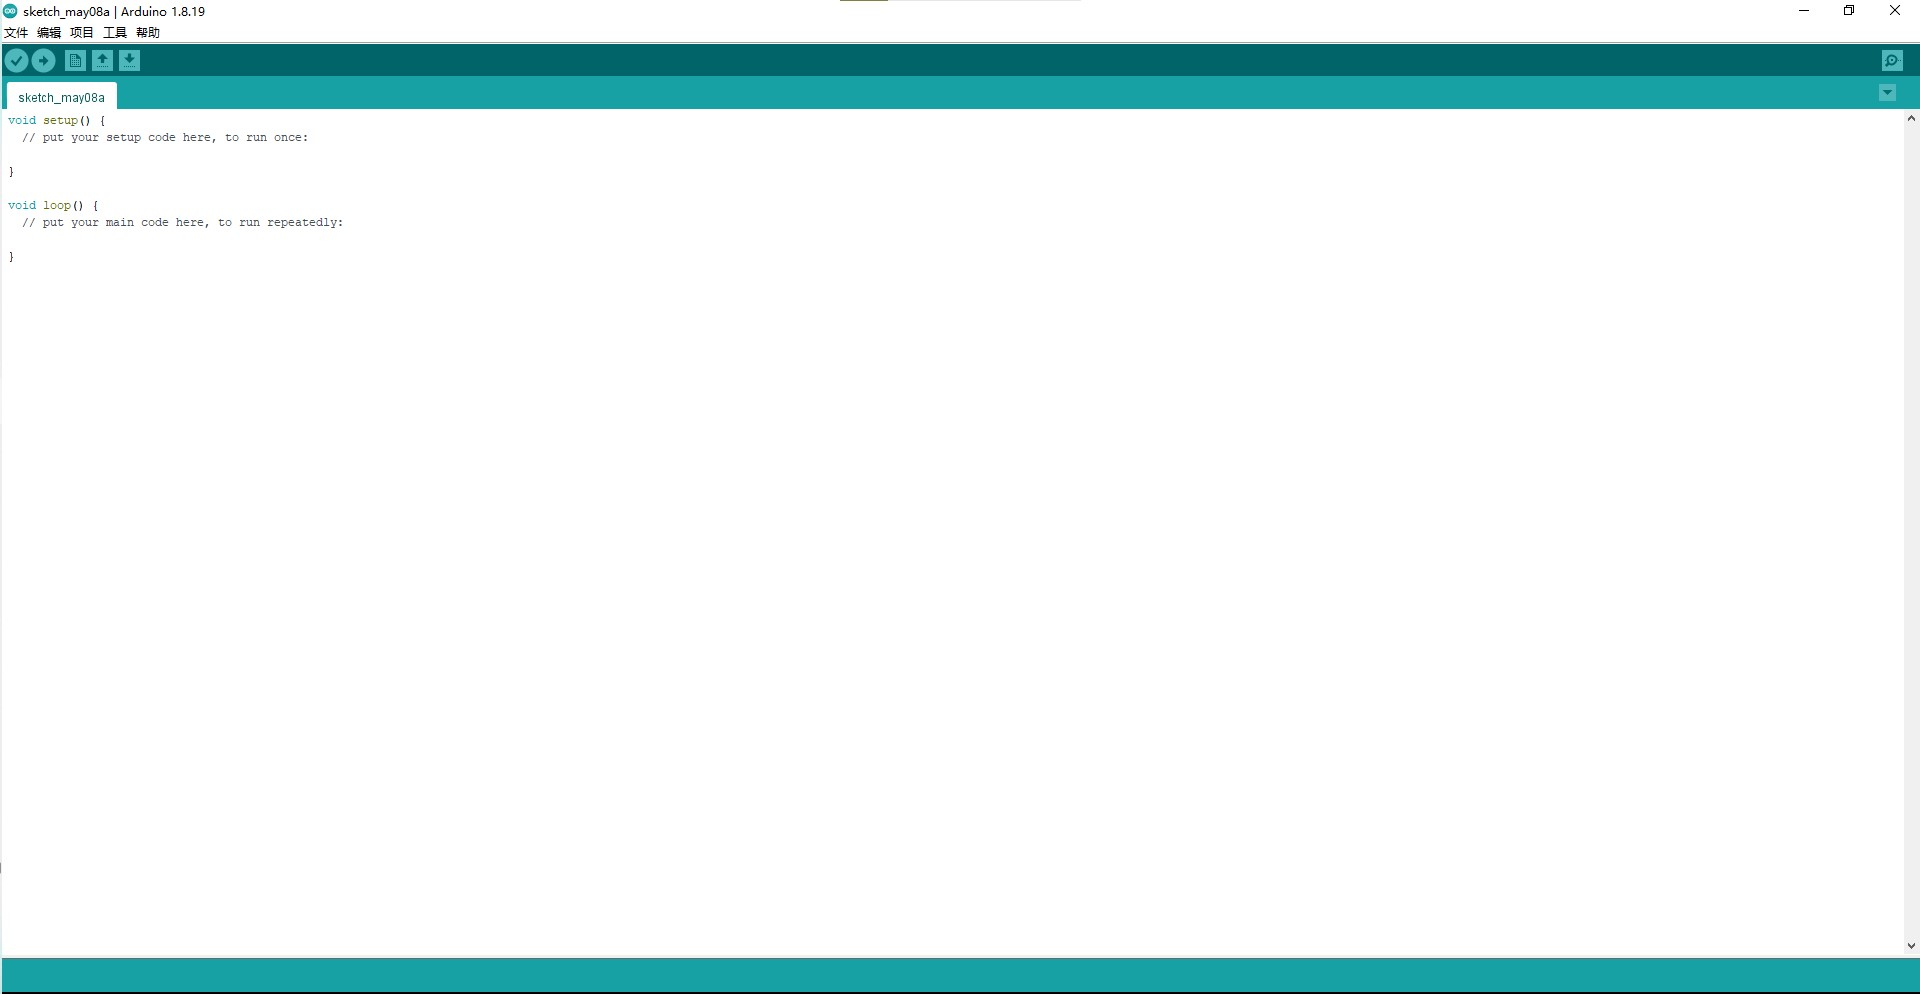
\includegraphics[width=0.60\textwidth]{Arduino_IDE.jpg}
  \end{center}
  \caption{\texttt{Arduino IDE}}
\end{figure}
%
\texttt{Arduino IDE}(Integrated Development Environment) 是一个跨平台的开发工具,支持 Windows、Mac 和 Linux 操作系统。
以下是\texttt{Arduino IDE}的一些主要特点和功能:
\begin{enumerate}
  \item 代码编辑器:\texttt{Arduino IDE}内置了一个代码编辑器,
    支持基于C/Cpp的编程。用户可以在编辑器中编写代码,
    并提供了代码高亮显示、自动补全、代码调试等功能。
  \item 串口监视器:\texttt{Arduino IDE} 提供了串口监视器功能,
    用户可以通过串口监视器查看开发板与计算机之间的通信数据,
    便于调试和查看程序输出信息。
  \item 库管理器:\texttt{Arduino IDE}集成了库管理器,用户可以方便地搜索、
    安装和更新各种库,这些库包含了许多常用的函数和代码示例,
    可以加快开发过程。
  \item 编译功能: 编译功能会将用户编写的代码进行预处理、
    编译和链接等过程,生成一个可执行文件(hex文件、bin文件),
    该文件包含了二进制形式的机器指令.
\end{enumerate}
%
\subsection*{安信可串口调试助手}
\begin{figure}[H]
  \begin{center}
    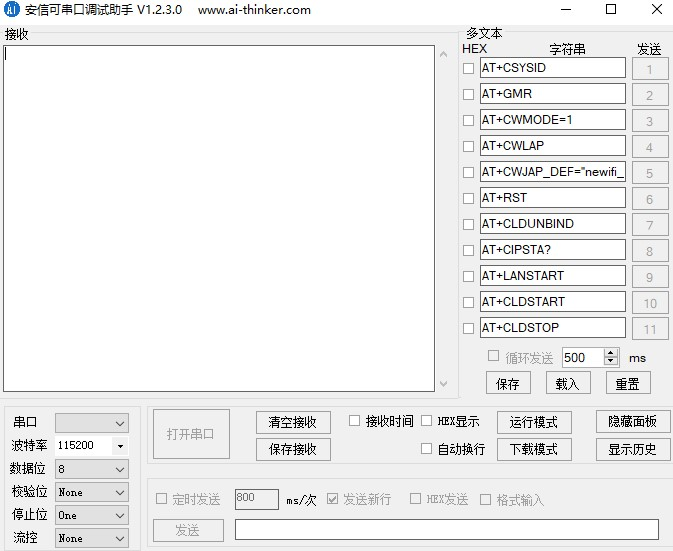
\includegraphics[width=0.35\textwidth]{ai-thinker_serial_tool.jpg}
  \end{center}
  \caption{\texttt{安信可串口调试助手}}
\end{figure}
%
\texttt{安信可窗口调试助手}是一款用于调试串口通信的软件工具。
它能够帮助开发人员在串口通信过程中监视数据的发送和接收,
进行调试和分析,从而提高开发效率和确保通信质量。

\texttt{安信可窗口调试助手}具有以下特点和功能:
\begin{itemize}
  \item \textbf{串口通信监控}:可以实时显示串口通信数据的发送和接收情况,
    包括数据内容、发送时间、接收时间等信息,方便用户了解通信过程。
  \item \textbf{数据格式化显示}:支持十六进制、ASCII等不同格式的数据显示,
    用户可以根据需要选择合适的显示方式,方便查看和分析数据。
  \item \textbf{数据记录与保存}:支持数据的记录和保存功能,
    用户可以保存通信过程中的数据以便后续分析和查看。
  \item \textbf{快捷设置}:提供简单易用的设置界面,用户可以快速配置串口参数,
    如波特率、数据位、校验位等。
\end{itemize}

\texttt{安信可窗口调试助手}在嵌入式系统开发、传感器调试、通信设备测试等领域具有广泛的应用。
通过使用该工具,开发人员可以更轻松地进行串口通信调试和故障排查,
提高开发效率,确保通信可靠性。
\subsection*{Flash Download Tool}
\begin{figure}[H]
  \begin{center}
    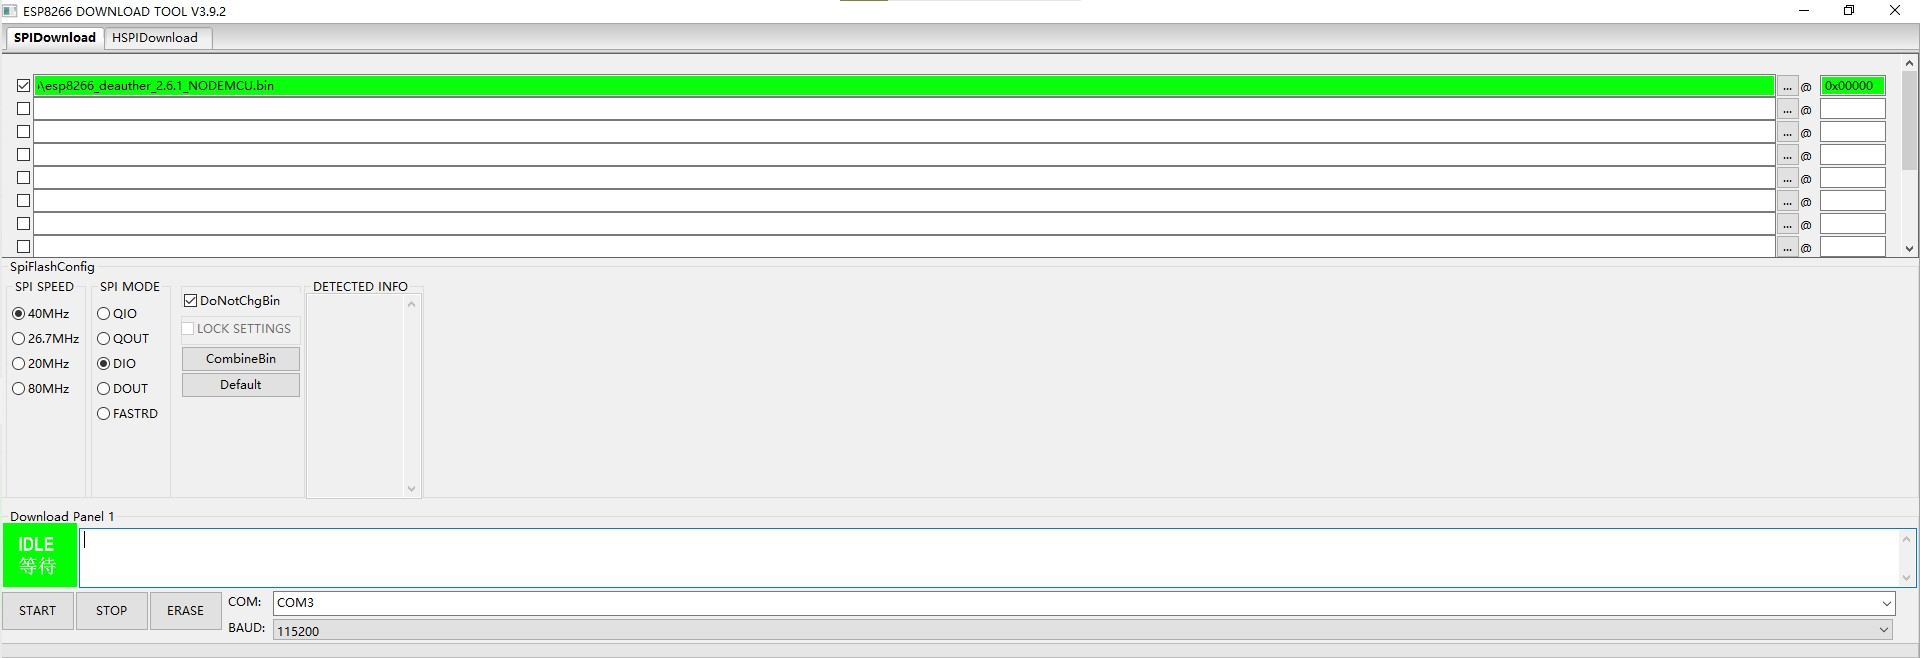
\includegraphics[width=0.45\textwidth]{flash_download_tool.jpg}
  \end{center}
  \caption{\texttt{Flash Download Tool}}
\end{figure}
%
使用时需要注意选择正确的波特率和下载地址.
%
\end{document}
